%%% This is the ISC-2020 Frankfurt 2st tutorial, B1

\MEchapter[High performance]{How to achieve high performance}
\MESetListingFormat[basicstyle={\ttfamily\color{black}\normalsize}]{SystemC}

%\subsubsection{How to achieve high performance 45+5'}
%The question of single-thread vs many-processor optimization
%is shortly touched.
%The need for using parallelized sequential processing is introduced
%and the general limitations of computing systems are recalled, 
%based on the model. As the model suggests, different contributions
%to the sequential-only portion of the tasks is detailed
%and their role in the final non-parallelizable portion is discussed.
%Based on some published technical data,
%the limiting effects of the technical implementations discussed.

\MEsection{Expectations}

\MEframe{What was expected in 15 year ago}
{
	The expectations are huge and excessive. Looking at Fig~\ref{Expectations2005},
	that the detailed expectations really need a high performance.
	it is worth to notice, however, that a slowdown and a saturation
	was expected to the years 2020-2030.
	\MEfigure{fig/ZettaflopsSandia}
	{Why hight performance is needed and what performance was expected in 2005}
	{Expectations2005}{}{.85}
}


\MEframe{What was expected 5 year ago}
{
	
	\MEfigure{fig/TOP500PerformanceDevelopment.png}
	{What perfromance was expected in 2015}
	{Expectations2015}{}{.85}
}

%
%\MEframe{What is expected in 2020}
%{
%	
%	\MEfigure[wide]{fig/PerfExpectations2019}
%	{What is experienced right now}
%	{Expectations2019}{}{}
%}

\MWframe{}
 {
 	
 }
 
\MEframe{What is experienced}
{
	
	\MEfigure{fig/SupercompSpeedOfLight.pdf}
	{The payload performances of some TOP500 supercomputers}
	{Reality2019}{}{.85}
}

https://sciencenode.org/feature/the-race-to-exascale.php

\MEsection[High performance]{How to achieve high performance}

\MEframe{Just a question of money, strategy and political will - 2016}
{
	\MEquote{	
		the largest HPC hardware systems today
		contain more than 1 million cores, and exascale
		supercomputers with tens or hundreds of millions
		of cores will begin to arrive during the period
		2020-2022 " and "With a differentiated strategy
		and sufficient investment and political will,
		Europe can be a global player in HPC.}
	{Europe Union’s Action plan, 2016)}
}	


\MEsection[The math]{Amdahl's Law}
\MEframe{The mathematics of Amdahl's Law}
{
	\only<1>
	{
		\MEquote{Everyone knows Amdahl's Law, but quickly forgets it.}{Thomas Puzak, IBM, 2007}
	}
	
	\only<2>
	{
		Usually,  Amdahl's law is expressed as 
		\vspace{-.3\baselineskip}	
		\begin{equation}
		S^{-1}=(1-\alpha) +\alpha/N \label{eq:AmdahlBase}
		\end{equation}
		
		\noindent where $N$ is the number of parallelized code fragments, 
		$\alpha$ is the ratio of the parallelizable fraction to the total,
		$S$ is the measurable speedup. 
		
		\vspace{-.3\baselineskip}	
		\begin{equation}
		\alpha = \frac{N}{N-1}\frac{S-1}{S} \label{equ:alphaeff}
		\end{equation}
		
		When calculating speedup, one actually calculates
		\vspace{-.3\baselineskip}	
		\begin{equation}
		S=\frac{(1-\alpha)+\alpha}{(1-\alpha)+\alpha/N} =\frac{N}{N(1-\alpha)+\alpha}
		\end{equation}
		hence  the \textit{efficiency}
		\vspace{-.3\baselineskip}	
		\begin{equation}
		\boxed{E(\large N,\alpha)} = \frac{S}{N}=\boxed{\frac{1}{\textcolor{webred}{\Large N}(1-\alpha)+\alpha}}= \frac{R_{Max}}{R_{Peak}} \label{eq:soverk}
		\end{equation}
	}
}

\MEsection{The efficiency surface}
\MEframe{Parallization efficacy as 2-parameter function}
{
	\vskip -.5cm
	\begin{figure}
		\maxsizebox{\textwidth}{.8\textheight}{
			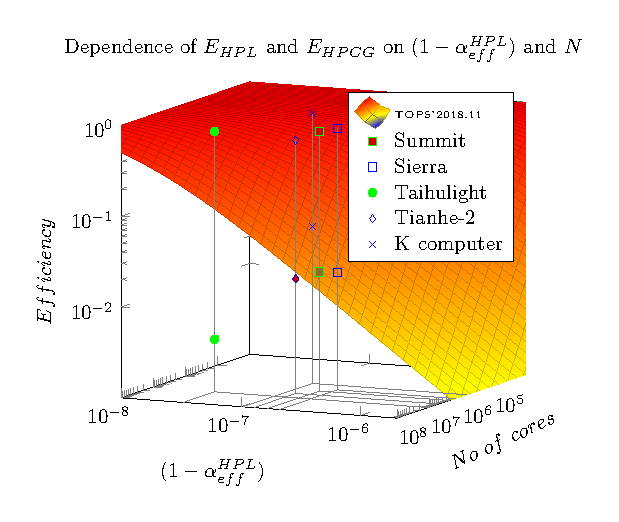
\includegraphics{fig/EffDependence2018LogA.pdf}
		}
	\end{figure}
	%	\pause
	{"The efficency is a feature rather than a bug".}
	
	%	\pause
	{”this decay in performance is not a fault of the
		architecture, but is dictated by the limited parallelism”.\cite{ScalingParallel:1993}}
}


\MEsection[The model]{Amdahl's model}
\MEframe{The model of parallel/sequential operation}
{
	\begin{figure}
		\maxsizebox{\textwidth}{.85\textheight}{
			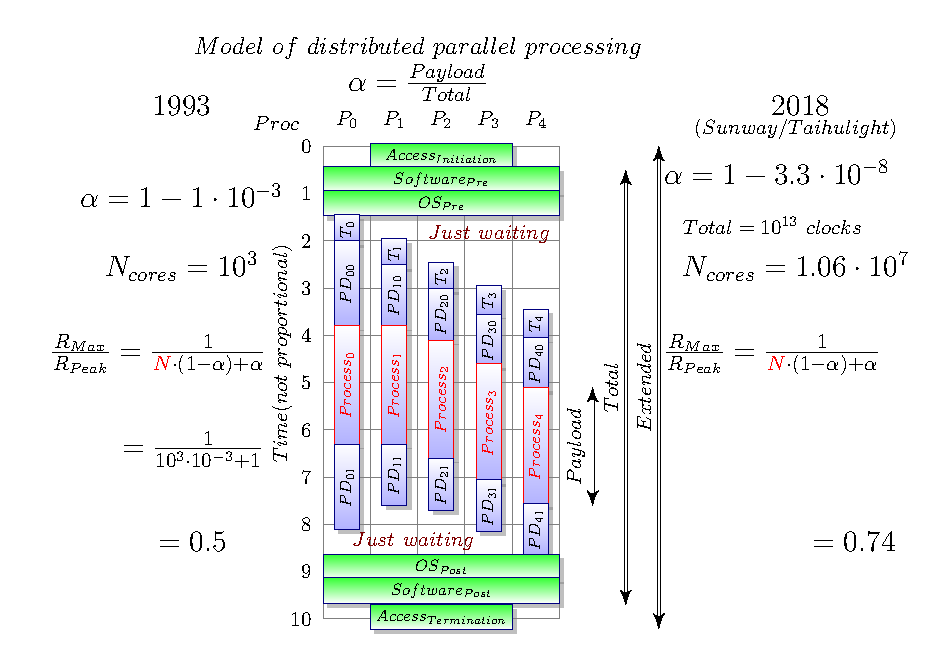
\includegraphics{fig/AmdahlModelAnnotated.pdf}
		}
	\end{figure}
	%	\pause
	\textbf{\textit{SW, \textcolor{red}{HW  and science} contribute to the sequential-only fraction.}}
	
	(The terms of the simple non-technical model need proper interpretation.)
}

